\documentclass{article}
    \usepackage{url}
    \usepackage{cite}
    \usepackage{float}   
    \usepackage{xcolor}
    \usepackage{lscape}
    \usepackage{amssymb}
    \usepackage{titling}
    \usepackage{pdfpages}
    \usepackage{enumitem}
    \usepackage{graphicx}
    \usepackage{hyperref}
    \usepackage{fancybox}
    \usepackage{fancyvrb}
    \usepackage{enumerate}
    \usepackage{pdflscape}
    \usepackage{afterpage}
    \usepackage{listings,lstautogobble}    
    \usepackage[margin=0.8in]{geometry}
    \usepackage[nottoc,notlot,notlof]{tocbibind}
    \renewcommand\maketitlehookd{\vfill\null}
    \renewcommand\maketitlehooka{\null\mbox{}\vfill}

    \newcommand\backgroundimage{
        \put(-5,0){
        \parbox[b][\paperheight]{\paperwidth}{
        \vfill
        \centering
        
\includegraphics[height=\paperheight]{Images/background.jpg}
        \vfill
    }}}

    % Stole code from: https://tex.stackexchange.com/questions/83882/how-to-highlight-python-syntax-in-latex-listings-lstinputlistings-command

    % Default fixed font does not support bold face
    \DeclareFixedFont{\ttb}{T1}{txtt}{bx}{n}{12} % for bold
    \DeclareFixedFont{\ttm}{T1}{txtt}{m}{n}{12}  % for normal

    \definecolor{deepblue}{rgb}{0,0,0.5}
    \definecolor{deepred}{rgb}{0.6,0,0}
    \definecolor{deepgreen}{rgb}{0,0.5,0}

    % SQL style for highlighting
    \lstset{
        language=SQL,
        basicstyle=\small,
        commentstyle=\color{gray},
        otherkeywords={self},
        keywordstyle=\ttb\color{deepblue},
        stringstyle=\color{deepgreen},
        numbers=left,
        numberstyle=\small,
        breaklines=true,
        frame=tb,
        showstringspaces=false,
        autogobble=true
        }

    \graphicspath{ {Images/} }

    \title{EBUS3030 Assignment 1}
    \author{
        Steven Karmaniolos 
        \texttt{c3160280@uon.edu.au}\\
        Jay Rovacsek
        \texttt{c3146220@uon.edu.au}\\
        Jacob Litherland
        \texttt{c3263482@uon.edu.au}\\
        Edward Lonsdale
        \texttt{c3252144@uon.edu.au}
    }
    \date{\today}
    \hypersetup{
    colorlinks=true,
    linkcolor=black,
    filecolor=magenta,      
    urlcolor=blue,
    citecolor=red,
    linktoc=section,
    }
    \pagenumbering{arabic}

    \newlist{legal}{enumerate}{10}
    \setlist[legal]{label*=\arabic*.}

    \begin{document}
    \AddToShipoutPicture{\backgroundimage}

    \begin{titlingpage}
        \maketitle
    \end{titlingpage}

    \tableofcontents

    \newpage

    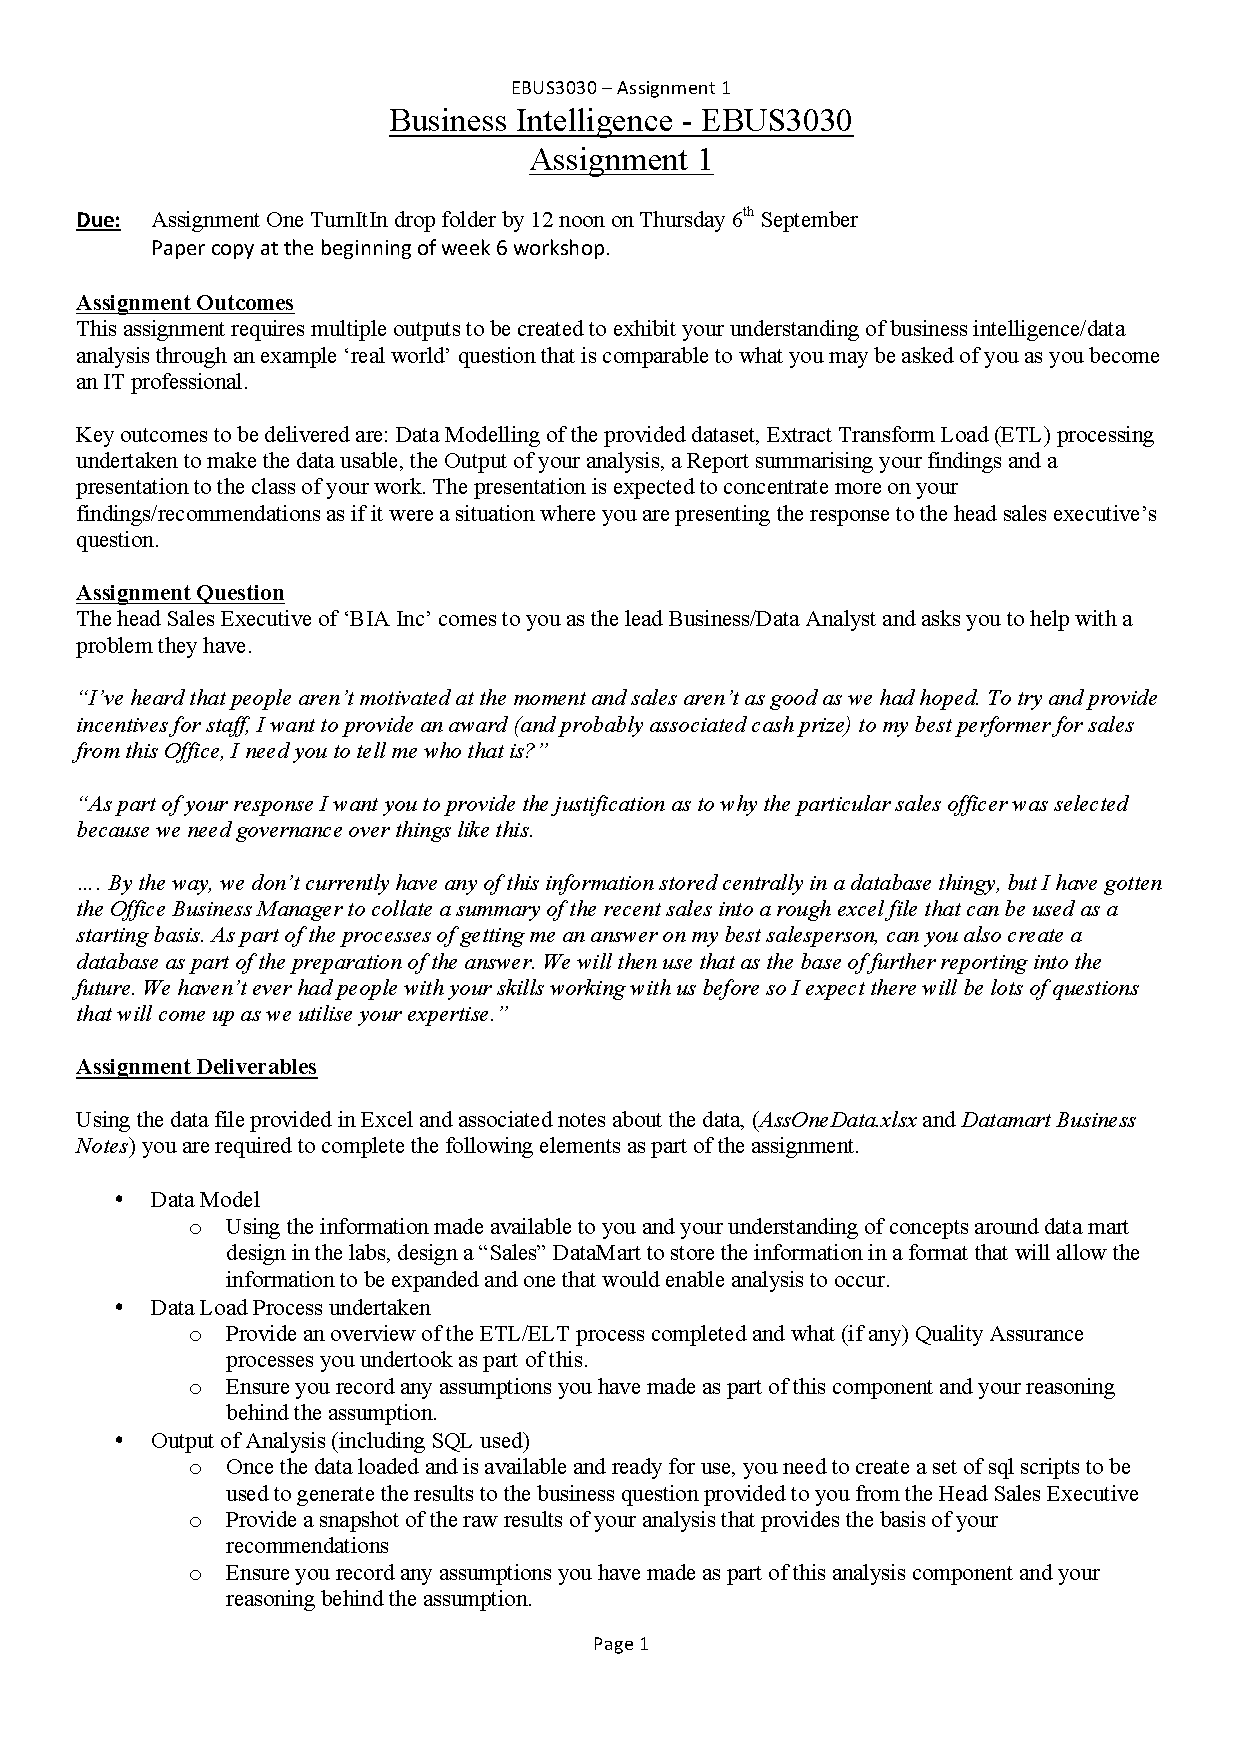
\includepdf[pagecommand=\section{Assignment Overview \& Requirements},width=\textwidth,keepaspectratio,pages={1}]{Resources/Assignment1Overview.pdf}
    \includepdf[width=\textwidth,keepaspectratio,pages={2}]{Resources/Assignment1Overview.pdf}

    \subsection{Datamart Business Rules}
    The following business rules were provided to be used in the context of this assignment:
    \begin{itemize}
        \renewcommand\labelitemi{*}
        \item At BIA all customers interacts are in an online environment, 
        there are no orders outside of electronic.
        \item Returning customers can provide POI information via the web
        interface and look up their record and that will flow with the sale.
        \item The sales associate can complete the order form/sale for the
        client.
        \item Each sale will have a receipt number/id.
        \item A receipt can have many line items.
        \item Each line item can only be for a single item, but the customer can
        purchase multiples of the same item.
        \item Where a customer has multiple line items, any sale with more than
        5 row items (containing at least 5 different items) is provided a
        15\% discount.
        \item The system automatically handles the total for the sale by looking
        up the item, then multiplying the costs per item by number
        purchased, and then should store this final field total as a record
        in the system (but should also be able to see clearly sales that
        were provided a discount.
        \item Item prices can change at any point, and the price the customer
        pays is the amount listed for the item on the sale date. We need to
        keep a record of all item prices historically.
        \item Only 1 BIA sales assistant can be attributed to any receipt.
    \end{itemize}

    With these considerations in mind, the following report was created to outline
    the discovery, creation and polish to satisfy the assignment requirements.

    \newpage
    \section{Data Model}
    The below data model is only a suggestion and is still subject to change into the future. A full create script can be found in the \hyperref[sec:Appendix]{\color{blue}appendix}
        \begin{center}
            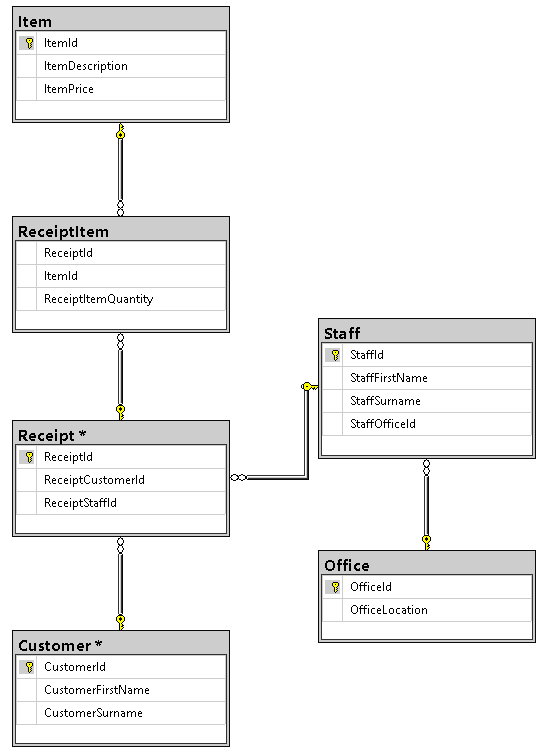
\includegraphics[width=\textwidth]{Images/Suggested_Schema.PNG}
        \end{center}
    It must be noted that the structure of this data model is 
    less than efficient, and it would be expected in a datamart
    situation that only at lower levels of data would this schema
    remain responsive in the manner it is now, as the outline
    suggests the datamart is not necessarily the most suitable
    design for future use, however suits very well currently.
    \par
    It would be expected that only at extremely large data sets
    would this model prove a bad design. In such cases a model 
    more representative of the snowflake or star schema would be
    heavily advised.

    \newpage
    \section{Data Load Process (ETL/ELT)}
        Initial import of the data supplied in the xlsx file generated a very basic table
        that allowed us to analyze the data for potential outliers, confirm the business
        requirements of the data and then create tables from which the data model was derived.
        \\
        The Imported table structure was as follows:
        \begin{center}
            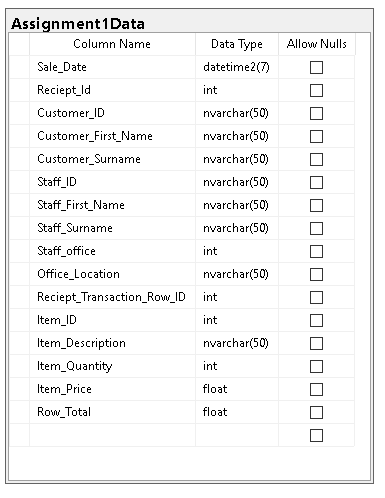
\includegraphics{Images/Initial_Import.PNG}
        \end{center}

        A decision to leave this initial import table as default
        was made to allow easy reference to the initially supplied
        excel data file.
        \par
        In the following sections of \hyperref[sec:QAP]{\color{blue}Quality Assurance Processes}, \hyperref[sec:AR]{\color{blue}Assumptions and Reasoning} and \hyperref[sec:BA]{\color{blue}Base Analysis} we intend to clarify the reasoning behind leaving the imported data in
        the default table suggested by SSMS.

        \newpage

        \subsection{Quality Assurance Processes}
        \label{sec:QAP}
            A number of queries were written to look for data which did not adhere to the spec
            outlined in business requirements and to ensure data was "clean" before entry.
            The first instance of potential issues were encountered with a basic \hyperref[sec:Python]{\color{blue}python} script
            which checked validity of column data, it was found that cells starting at B13777
            to the end of file in the originally supplied excel file were formula values and 
            not static values, this would not have caused an issue with importing into SSMS 
            however certainly broke the script temporarily.
            \par
            After clarifying the issues with the aforementioned cells with Peter, a data file without
            the offending formula was supplied and used for the remainder of the assignment.
            \vspace{5mm}
            \par\noindent
            The next potential issue encountered was not until a suggested schema structure 
            was complete and data was being scripted to be added to the new schema for analysis.
            The issue encountered was that receipt number 52136 seemed to be an incorrect 
            entry, this was discovered when running the import query for the new schema:

            \begin{lstlisting}
                INSERT INTO Receipt(ReceiptId, ReceiptCustomerId,ReceiptStaffId)
                SELECT DISTINCT(Reciept_Id),Customer_ID,Staff_ID
                FROM Assignment1Data
                ORDER BY Reciept_Id
            \end{lstlisting}

            Which resulted in the error:
            \color{red}
            \begin{Verbatim}[fontsize=\small]
    Violation of PRIMARY KEY constraint 'PK_Receipt'. Cannot insert duplicate key in object 
    'dbo.Receipt'. The duplicate key value is (52136).
            \end{Verbatim}
            \color{black}

            Leading us to recognise that either one of the entries could be incorrect, therefore
            best to investigate both records of the customer Id against the rest of the database:

            \begin{lstlisting}
                SELECT * FROM Assignment1Data 
                WHERE Customer_ID='C32' 
                AND Staff_ID='S15' 
                AND Sale_Date='2017-11-12 00:00:00.0000000';
            
                SELECT * FROM Assignment1Data 
                WHERE Customer_ID='C13' 
                AND Staff_ID='S4' 
                AND Sale_Date='2017-12-30 00:00:00.0000000';
            \end{lstlisting}

            When both queries were performed it was apparent that the data associated with C32 was 
            the likely broken record and modification of the data occurred:

            \begin{lstlisting}
                UPDATE Assignment1Data 
                SET Reciept_Id=51585, 
                Reciept_Transaction_Row_ID=(
                    SELECT MAX(Reciept_Transaction_Row_ID)+1 
                    FROM Assignment1Data
                    WHERE Reciept_Id=51585)
                WHERE Customer_ID='C32' 
                AND Staff_ID='S15' 
                AND Sale_Date='2017-11-12 00:00:00.0000000' 
                AND Item_ID='14';
            \end{lstlisting}

            The next issue arose when again, attempting to run the aforementioned query to import
            into the new Receipt table, this time not one stray record was found, but a complete
            collision on the ReceiptId of 52137, this time as neither record seemed to have 
            records that were correct, it was decided to move one to the maximum ReceiptId + 1:

            \begin{lstlisting}
                UPDATE Assignment1Data 
                SET Reciept_Id=(
                    SELECT MAX(Reciept_Id)+1 
                    FROM Assignment1Data) 
                WHERE Customer_ID='C27' 
                AND Staff_ID='S4' 
                AND Sale_Date='2017-12-30 00:00:00.0000000';
            \end{lstlisting}

            The same issue was replicated on ReceiptId 52138, resolved via:

            \begin{lstlisting}
                UPDATE Assignment1Data 
                SET Reciept_Id=(
                    SELECT MAX(Reciept_Id)+1 
                    FROM Assignment1Data) 
                WHERE Customer_ID='C30' 
                AND Staff_ID='S19' 
                AND Sale_Date='2017-05-16 00:00:00.0000000';
            \end{lstlisting}

            At this point we recognised the broken data likely continued for a while, and 
            evaluated our hypothesis by looking at the original excel file. It turned
            out that data with ReceiptId from 52137-52145 was all broken in the same manner.
            The following query shows this well:

            \begin{lstlisting}
                SELECT Reciept_Id, Customer_ID,Staff_ID 
                FROM Assignment1Data 
                WHERE Reciept_Id BETWEEN 52137 AND 52150
                GROUP BY Reciept_Id, Customer_ID,Staff_ID 
                ORDER BY Reciept_Id;
            \end{lstlisting}

            In order to clean this data we looked at a number of potential methods, with an 
            emphasis on avoiding effort in the task if possible but not breaking the data further,
            which to this point just appeared to be a collision of a number of receipts.
            \\
            We knew a structure such as a CTE\cite{CTE} would allow us to easily split
            distinct records which shared a receiptId and filter by a value such as row number.

            \begin{lstlisting}
            WITH CTE AS
            (
                SELECT ROW_NUMBER() OVER (ORDER BY Reciept_Id) AS RowNumber,
                        Reciept_Id,
                        Customer_ID,
                        Staff_ID
                FROM  Assignment1Data
                WHERE Reciept_Id BETWEEN 52137 AND 52150
                GROUP BY Reciept_Id, Customer_ID,Staff_ID 
            )
            SELECT Reciept_Id,Customer_ID,Staff_ID FROM CTE WHERE (RowNumber % 2 = 0)
            \end{lstlisting}

            Results of the above query yielded:
            \begin{table}[H]
                \centering
                \begin{tabular}{|l|l|l|}
                \hline
                Reciept\_Id & Customer\_Id & Staff\_Id \\ \hline
                52137       & C59          & S2        \\ \hline
                52138       & C30          & S19       \\ \hline
                52139       & C31          & S20       \\ \hline
                52140       & C52          & S10       \\ \hline
                52141       & C42          & S7        \\ \hline
                52142       & C47          & S6        \\ \hline
                52143       & C8           & S13       \\ \hline
                52144       & C50          & S4        \\ \hline
                52145       & C40          & S15       \\ \hline
                52146       & C38          & S5        \\ \hline
                52147       & C9           & S19       \\ \hline
                52148       & C43          & S16       \\ \hline
                52149       & C45          & S11       \\ \hline
                52150       & C57          & S7        \\ \hline
                \end{tabular}
            \end{table}

            \newpage
            
            Whereas the original result without a modulo comparison on the row would have yielded
            a much different result, the raw table supplied in the \hyperref[sec:CTEResults]{\color{blue}appendix}
            \par
            With this known, and additional section was added to the \hyperref[sec:Python]{\color{blue}python} script to generate update statements
            that would be easy to add to the current migrations.sql script we were prototyping.
            \\
            The generated update statements appeared as:

            \begin{lstlisting}
                -- Auto-generated query to fix error of type: Staff.Id Mismatch
                -- Resolved error identified by UUID: dcf16fba08c63ecc85556c385204d9524ec359cf
                UPDATE Assignment1Data 
                SET Reciept_Id=(
                SELECT MAX(Reciept_Id)+1 
                FROM Assignment1Data)
                WHERE Reciept_Id=52136
                AND Customer_Id = 'C13' AND Staff_Id = 'S4'
                GO
            \end{lstlisting}

            Determining now potential entries that broke further rules was our next objective.
            We pursued the idea that entries of receipts could potentially have duplicate items
            recorded against the ReceiptItem table. A simple script was generated to check our 
            assumptions of this:

            \begin{lstlisting}
                -- Verify that no receipt has duplicate ItemIds and all are unique per order
                SELECT *
                FROM
                (
                    SELECT [ReceiptItem].[ReceiptId], 
                    COUNT([ReceiptItem].[ReceiptId]) AS 'ItemCount',
                    COUNT(DISTINCT [ReceiptItem].[ItemId]) AS 'ItemIdCount'
                    FROM [ReceiptItem]
                    GROUP BY [ReceiptItem].[ReceiptId]) AS SubQuery 
                WHERE [SubQuery].[ItemIdCount] != [SubQuery].[ItemCount]
                ORDER BY [SubQuery].[ReceiptId]
                GO
            \end{lstlisting}

            This query returned a result of 912 rows out of the total 2514, which we believed 
            was a large amount given the issues identified earlier numbered in only the teens, 
            however on manual inspection of a number of the reported issue records, it was 
            apparent this figure was actually correct. 
            \par
            Given the large task associated with the entries, an additional module was
            written for generation of SQL in \hyperref[sec:Python]{\color{blue}python} which resulted in two queries for each
            duplicate item entry per receipt, the first query updating the total of one of the 
            records to reflect the real item quantity, the later dropping the non-altered 
            entry after the first had been completed.

            \newpage

            The script was as follows:
            \begin{lstlisting}
                -- Auto-generated query to fix error of type: Item.Id Duplicate
                -- Resolved error identified by UUID: 0ee74976129cce87fb1558eb5586b1511f5c8d8f
                UPDATE Assignment1Data 
                SET [Item_Quantity]=(
                SELECT SUM([Item_Quantity])
                FROM Assignment1Data
                WHERE Reciept_Id=51500
                AND Item_ID = 20)
                WHERE Reciept_Id=51500
                AND Item_ID = 20
                AND Item_Quantity = 1
                GO

                -- Auto-generated query to fix error of type: Item.Id Duplicate
                -- Resolved error identified by UUID: 0ee74976129cce87fb1558eb5586b1511f5c8d8f
                DELETE FROM Assignment1Data 
                WHERE Reciept_Id=51500
                AND Item_ID = 20
                AND Item_Quantity < 1
                GO
            \end{lstlisting}

            Having now cleaned what we believed to be all discrepancies, we could finally start to look at
            evaluating data, our analysis outlined in \hyperref[sec:BA]{\color{blue}base analysis}
        \newpage
        \subsection{Assumptions and Reasoning}
        \label{sec:AR}
            \subsubsection{Item Table}
                An assumption of the ItemId never needing to be larger than a smallint
                was followed, as a basic query into the maximum range within the test data
                suggested that the maximum Id that currently existed was 30:
                \begin{lstlisting}
                    -- Some basic queries for us to determine potential outlier data:
                    -- What is the max of each column where datatype is int?
                    SELECT MAX(Item_ID) AS 'Max Item_ID'
                    FROM Assignment1Data;
                \end{lstlisting}

                With the results:

                \begin{Verbatim}[fontsize=\small]
    Max Item_ID
    30
                \end{Verbatim}
                ItemDescription underwent some size optimisation, as the max data length 
                that currently existed within the supplied data was 52, and we are to assume
                that into the future more items may be added, a value of 255 should allow
                for a varied range of descriptions.
                \\
                SQL queried to determine to above assumption:

                \begin{lstlisting}
                    -- Determine current max varchar used in Item_Description
                    SELECT MAX(DATALENGTH(Item_Description)) 
                    FROM Assignment1Data;
                \end{lstlisting}

                We do recognise the requirements for optimisation may not require such measures, and 
                acknowledge that a varchar(max)/text datatype would also be reasonable.
            \subsubsection{Price Table}
                The price table was designed to hold historical data as required by the business rules,
                an effective range can be used here to determine item pricing for time frames,
                current items having no end date or an end date as some point in time into the future.
                \par
                Accuracy on the pricing was important, we decided to use a decimal(19,5) structure to
                ensure no problems should arise at any point with calculation of totals.\cite{MoneyIssues}
            \subsubsection{ReceiptItem}
                The receipt item table acts as a line-item style associative entity, the quantity and 
                historical priceId used at time of transaction can allow an item's price to be
                updated and still maintain historical pricing associated with the receipt.
            \subsubsection{Receipt}
                The receipt table acts as a meta-table in this instance, other tables associate with 
                this table with the receiptId field. Due to this it made it extremely easy to use a number
                of joins/inner joins to determine some of the metrics outlined in the \hyperref[sec:BA]{base analysis}.
            \subsubsection{Staff}
                Staff was left in a non-normalised state to ensure efficiency of queries into the future, 
                normalising the table further would yield little value to the business based on the requirements.
                The office table is referenced by the staff table. This is merely to satisfy the assumption
                that, while the only office to exist was Newcastle in this setting, the requirement of more 
                offices into the future is a possibility and the required join would be little impact on speed
                of queries in a datamart.
            \subsubsection{Customer}
                Customer, just like staff could be normalised further requiring more joins and potentially 
                causing a performance issue into the future, for simplicity we kept only the supplied
                data in mind, and assumed no more data would be required by the datamart into the future.

    \section{Base Analysis}
    \label{sec:BA}
        \subsection{Raw Results}
            A number of metrics were considered to satisfy the request related to the best salesperson,
            as we are not certain if this is determined by a specific metric or a set of metrics we 
            included a number of analyzed points for the project:
            \begin{itemize}
                \item Total receipts attributed to a staff member
                \item Total items sold by a staff member
                \item Ratio of discounted sales to normal sales for each staff member
                \item Total sale value per staff member
                \item Average sale value per staff member
                \item Average item value per staff member
            \end{itemize}

            \subsubsection{Total Number of Sales}
                The total number of sales per staff member were considered with the following 
                sql query:
                \begin{lstlisting}
                    -- Sales count per staff member (Receipt Count)
                    SELECT COUNT(*) AS 'Sales Count', s.StaffId,s.StaffFirstName,s.StaffSurname
                    FROM Receipt r
                    INNER JOIN ReceiptItem ri ON r.ReceiptId = ri.ReceiptId
                    INNER JOIN Item i ON i.ItemId = ri.ItemId
                    INNER JOIN Price p ON p.PriceId = ri.PriceId
                    INNER JOIN Staff s ON s.StaffId = r.ReceiptStaffId
                    GROUP BY s.StaffId,s.StaffFirstName,s.StaffSurname
                    ORDER BY 'Sales Count' DESC;
                \end{lstlisting}

                Leading to a range of 736 to 500, the top five staff were:

                \begin{table}[H]
                    \centering
                    \begin{tabular}{|l|l|l|l|}
                    \hline
                    Sales Count & StaffId & StaffFirstName & StaffSurname \\ \hline
                    736         & S17     & Daniel         & Baker        \\ \hline
                    709         & S19     & Kaitlyn        & Ortiz        \\ \hline
                    702         & S8      & Michelle       & Miller       \\ \hline
                    701         & S1      & Lauren         & Martin       \\ \hline
                    700         & S5      & Stephanie      & Watson       \\ \hline
                    \end{tabular}
                \end{table}
            \newpage
            \subsubsection{Total Items Sold}
                The total items attributed to each staff member were considered also,
                determined by the query:
                
                \begin{lstlisting}
                    -- Item count per staff member
                    SELECT SUM(ri.ReceiptItemQuantity) AS 'Item Count', s.StaffId,s.StaffFirstName,s.StaffSurname
                    FROM Receipt r
                    INNER JOIN ReceiptItem ri ON r.ReceiptId = ri.ReceiptId
                    INNER JOIN Staff s ON s.StaffId = r.ReceiptStaffId
                    GROUP BY s.StaffId,s.StaffFirstName,s.StaffSurname
                    ORDER BY 'Item Count' DESC;
                \end{lstlisting}

                Yeilding a range of 4481 to 2960, with the top five staff members in this
                analysis:
                \begin{table}[H]
                    \centering
                    \begin{tabular}{|l|l|l|l|}
                    \hline
                    Item Count & StaffId & StaffFirstName & StaffSurname \\ \hline
                    4481       & S17     & Daniel         & Baker        \\ \hline
                    4414       & S19     & Kaitlyn        & Ortiz        \\ \hline
                    4373       & S1      & Lauren         & Martin       \\ \hline
                    4333       & S8      & Michelle       & Miller       \\ \hline
                    4308       & S5      & Stephanie      & Watson       \\ \hline
                    \end{tabular}
                \end{table}
            \subsubsection{Discounted Sales Ratio}
            Consideration of the number of sales made by each staff member was also made,
            the following query yeilding the results we required:

            \begin{lstlisting}
                -- Sales metrics for discounted and standard sales per staff member
                SELECT s.StaffId,s.StaffFirstName,s.StaffSurname,
                SUM(SubQuery.[Discounted Sales]) AS 'Discounted Sales',
                SUM(SubQuery.[Standard Sales]) AS 'Standard Sales'
                FROM (
                    SELECT CAST(
                        CASE
                        WHEN COUNT(ri.[ReceiptItemQuantity]) >= 5
                            THEN 1
                        ELSE 0
                        END AS int) AS 'Discounted Sales',
                    CAST(
                        CASE
                        WHEN COUNT(ri.[ReceiptItemQuantity]) >= 5
                            THEN 0
                        ELSE 1
                    END AS int) AS 'Standard Sales',
                    r.ReceiptId
                    FROM Receipt r
                    INNER JOIN ReceiptItem ri ON r.ReceiptId = ri.ReceiptId
                    INNER JOIN Item i ON i.ItemId = ri.ItemId
                    INNER JOIN Price p ON p.PriceId = ri.PriceId
                    GROUP BY r.ReceiptId
                ) AS SubQuery
                INNER JOIN Receipt r ON SubQuery.ReceiptId = r.ReceiptId
                INNER JOIN ReceiptItem ri ON r.ReceiptId = ri.ReceiptId
                INNER JOIN Staff s ON s.StaffId = r.ReceiptStaffId
                GROUP BY s.StaffId,s.StaffFirstName,s.StaffSurname
            \end{lstlisting}

            \newpage
            Results from the query yielded:
            \begin{table}[H]
                \begin{tabular}{|l|l|l|l|l|l|}
                \hline
                StaffId & StaffFirstName & StaffSurname & Discounted Sales & Standard Sales & Discounted Sales Rate \\ \hline
                S4      & Robert         & Wood         & 559              & 102            & 84.57\%               \\ \hline
                S20     & Dylan          & Hall         & 563              & 112            & 83.41\%               \\ \hline
                S1      & Lauren         & Martin       & 584              & 117            & 83.31\%               \\ \hline
                S16     & Jordan         & Turner       & 561              & 117            & 82.74\%               \\ \hline
                S14     & Noah           & Brooks       & 565              & 118            & 82.72\%               \\ \hline
                S17     & Daniel         & Baker        & 603              & 133            & 81.93\%               \\ \hline
                S13     & Molly          & Carter       & 556              & 128            & 81.29\%               \\ \hline
                S5      & Stephanie      & Watson       & 567              & 133            & 81.00\%               \\ \hline
                S15     & Bailey         & Green        & 529              & 126            & 80.76\%               \\ \hline
                S6      & Evan           & Hill         & 562              & 137            & 80.40\%               \\ \hline
                S10     & Jonathan       & Jenkins      & 478              & 119            & 80.07\%               \\ \hline
                S18     & Megan          & James        & 540              & 137            & 79.76\%               \\ \hline
                S19     & Kaitlyn        & Ortiz        & 561              & 148            & 79.13\%               \\ \hline
                S7      & Molly          & Jackson      & 499              & 138            & 78.34\%               \\ \hline
                S9      & Mélissa        & Garcia       & 510              & 148            & 77.51\%               \\ \hline
                S8      & Michelle       & Miller       & 541              & 161            & 77.07\%               \\ \hline
                S2      & Joseph         & Reed         & 494              & 153            & 76.35\%               \\ \hline
                S11     & Gavin          & Thompson     & 424              & 135            & 75.85\%               \\ \hline
                S12     & Leah           & Harris       & 376              & 124            & 75.20\%               \\ \hline
                S3      & Amber          & Hill         & 435              & 157            & 73.48\%               \\ \hline
                \end{tabular}
            \end{table}
    \newpage
    \section{Executive Summary}
    This report was created for the head sales executive of BIA Inc, 
    in regard to which sales staff member was considered the best performer 
    based on the given data. As no specific metric was given for the task 
    of determining the best performer an analysis was performed, in order 
    perform this task the data was cleaned, reviewed and queried.
    \par\noindent
    The best sales officer in regards to the analysis of total number 
    of sales was Daniel Baker. 
    \\
    Mr Baker had made the largest number of 
    sales in the 12 months of data that was supplied with a total of 
    736 total sales counts. From this data it can also be seen that 
    after Mr Baker is Kaitlyn Ortiz with 709 total number of sales 
    (difference of 27).
    \vspace{5mm}
    \par\noindent
    The best sales officer in regards to the analysis of Total items 
    sold was also Daniel Baker. In the 12 months of data that was 
    supplied it can be seen that in Mr Baker’s 736 total sales, he 
    sold 4481 items. This is only a 67 item difference between Mr 
    Baker and second place Kaitlyn Ortiz who had a total of 4414. 
    \vspace{5mm}
    \par\noindent
    After considering theses analytics and reviewing the results 
    it can be seen that Mr Daniel Baker may be considered the best 
    sales officer in terms of Total sales and items sold and should 
    be eligible for the reward that is being discussed. 

    \newpage
    \begin{thebibliography}{9}
        \raggedright
        \bibitem{MoneyIssues}
            Reasons against TSQL Money type: Stackoverflow User; \textit{SQLMenace}
            \url{https://stackoverflow.com/questions/582797/should-you-choose-the-money-or-decimalx-y-datatypes-in-sql-server}
        \bibitem{Numeric}
            Microsoft TSQL documentation of Decimal/Numeric types
            \url{https://docs.microsoft.com/en-us/sql/t-sql/data-types/decimal-and-numeric-transact-sql?view=sql-server-2017}
        \bibitem{CTE}
        Microsoft documentation: WITH common\_table\_expression (Transact-SQL)
            \url{https://docs.microsoft.com/en-us/sql/t-sql/queries/with-common-table-expression-transact-sql?view=sql-server-2017}
    \end{thebibliography}

    \newpage
    \section{Appendix}
    \label{sec:Appendix}
    \subsection{CTE Raw Results}
    \label{sec:CTEResults}
    \begin{table}[H]
        \centering
        \begin{tabular}{|l|l|l|}
        \hline
        Reciept\_Id & Customer\_Id & Staff\_Id \\ \hline
        52137       & C27          & S4        \\ \hline
        52137       & C59          & S2        \\ \hline
        52138       & C29          & S13       \\ \hline
        52138       & C30          & S19       \\ \hline
        52139       & C3           & S5        \\ \hline
        52139       & C31          & S20       \\ \hline
        52140       & C38          & S4        \\ \hline
        52140       & C52          & S10       \\ \hline
        52141       & C24          & S19       \\ \hline
        52141       & C42          & S7        \\ \hline
        52142       & C46          & S8        \\ \hline
        52142       & C47          & S6        \\ \hline
        52143       & C51          & S17       \\ \hline
        52143       & C8           & S13       \\ \hline
        52144       & C11          & S10       \\ \hline
        52144       & C50          & S4        \\ \hline
        52145       & C21          & S8        \\ \hline
        52145       & C40          & S15       \\ \hline
        52146       & C38          & S16       \\ \hline
        52146       & C38          & S5        \\ \hline
        52147       & C40          & S18       \\ \hline
        52147       & C9           & S19       \\ \hline
        52148       & C26          & S8        \\ \hline
        52148       & C43          & S16       \\ \hline
        52149       & C10          & S19       \\ \hline
        52149       & C45          & S11       \\ \hline
        52150       & C15          & S10       \\ \hline
        52150       & C57          & S7        \\ \hline
        \end{tabular}
    \end{table}

    \newpage
    \subsection{Python Script}
    \label{sec:Python}

    % Python style for highlighting
    \newcommand\pythonstyle{\lstset{
        language=Python,
        basicstyle=\ttm,
        otherkeywords={self},
        keywordstyle=\ttb\color{deepblue},
        emph={
            Item,
            Office,
            Staff,
            Customer,
            Receipt,
            Sale,
            Sales,
            Employees,
            Items,
            Error_Log,
            Customers,
            LoggedErrors,
            __init__,
            },
        emphstyle=\ttb\color{deepred},
        stringstyle=\color{deepgreen},
        breaklines=true,
        frame=tb,
        showstringspaces=false
        }}
    
        % Python environment
        \lstnewenvironment{python}[1][]
        {
        \pythonstyle
        \lstset{#1}
        }
        {}
    
        % Python for external files
        \newcommand\pythonexternal[2][]{{
            \pythonstyle
            \lstinputlisting[#1]{#2}}}

    \begin{center}
        \pythonexternal{Data_Analysis/Scripts/parsedata/main.py}
    \end{center}

    \newpage

    \begin{center}
        \pythonexternal{Data_Analysis/Scripts/parsedata/classes.py}
    \end{center}
    
    \end{document}